\section{Models}

Keeping in mind that the discrepancy of the proton-charge radius is about $4\%$, we must be interested in rather small couplings \cite{Carlson:2015jba}.
Our primary model of interest is the addition of a scalar, $\phi$, with a weak, asymmetric coupling to leptons violating lepton universality.
We are also interested in the dark photon model, as it provides a similar low mass mediator that is weakly coupled to leptons.
In the dark photon model, this is instead a vector as opposed to a scalar.

\subsection{Dark Photon}
The dark photon model adds a new $U(1)'$ force where the mediator now carries a mass.
Giving the dark photon, known as the $A'$ (or alternatively the $V$), a kinetic mixing with the photon, allows it to couple to charged particles with a strength depending on the mixing strength.
This model has been thoroughly examined in the literature in connection with dark matter physics, and is a fairly general extension to the SM \cite{Holdom:1985ag}.
It also has potential to solve the $(g-2)_\mu$ problem \cite{Pospelov:2008zw}, however, more recently the parameter space for the simplest model has effectively closed off the dark photon as a solution to $(g-2)_\mu$ \cite{Batley:2015lha}.

The simplest version of the dark photon Lagrangian is given below in equation \ref{eqn:darkphoton_lagrangian}:
\begin{equation}
\label{eqn:darkphoton_lagrangian}
\Lagr = -\frac{1}{4}F'^2_{\mu\nu} + \frac{1}{2}m_{A'}^2 A'^2_\mu - \frac{\epsilon}{2}F'_{\mu\nu} F^{\mu\nu} + \Lagr_{\textrm{SM}}
\end{equation}
Here $F'_{\mu\nu} \equiv \partial_\mu A'_\nu - \partial_\nu A'_\mu$ is the field strength tensor corresponding to the dark photon vector field $A'_\mu$, $F_{\mu\nu}$ is the typical QED electromagnetic field strength tensor, $m_{A'}$ is the corresponding dark photon mass, and $\epsilon$ is the kinetic mixing strength.
The mass term appearing here actually could be inserted from a new Higgs field breaking the $U(1)'$ symmetry, and the QED field strength tensor replaced with the $F^Y_{\mu\nu}$ tensor from the SM $U(1)^Y$ electroweak group.
From a phenomenological point of view, it is sufficient to leave the mass term as it appears for our purposes.

After integrating the kinetic mixing term appearing in the Lagrangian by parts, the coupling to charged leptons (and quarks) becomes apparent as:
\begin{equation}
    \label{eqn:darkphoton_qed_current}
    \Lagr \supset \epsilon A'_\mu J^\mu_{EM}
\end{equation}
where $J^\mu_{EM} \equiv e \bar{\psi} \gamma^\mu \psi$ is the electromagnetic current.
We then have a coupling between fermions and the dark photon with strength $\epsilon e$, {\em i.e.}\ it looks just like the typical QED coupling but suppressed by a factor of $\epsilon$.
Taking the dark photon to decay to SM particles, we have the partial width of the dark photon to go to a lepton pair is given by,

\begin{equation}
    \Gamma_{A' \rightarrow \ell^+ \ell^-} = \frac{\alpha \epsilon^2}{3} m_{A'} \sqrt{1-\frac{4 m_\ell^2}{m_{A'}^2}}\left(1 + \frac{2 m_\ell^2}{m_{A'}^2}\right)
\end{equation}

\noindent which yields the convenient typical decay length when decaying to electrons to be given by \cite{Echenard:2014lma},

\begin{equation}
    c \tau_{A' \rightarrow e^+ e^-} \approx 0.8\textrm{mm} \left(\frac{10^{-4}}{\epsilon}\right)^2 \frac{10\textrm{MeV}}{m_{A'}}\textrm{.}
\end{equation}

\noindent One can see that for small $\epsilon$, the additional signature of the $A'$ could be its displace decay, away from the point where it has been produced.

In this model, the coupling to each lepton is the same.
It is not immediately clear that one can have an asymmetric effect across leptons on the charged proton radius, or the magnetic moment.
However in the case where a muon is concerned, the virtual particles may be much more massive.
For this reason, the muon is much more sensitive to undiscovered particles, such as an $A'$, than the electron, regardless of the couplings being the same between muon and electron.
The minimal model proved sufficient for an explanation of $(g-2)_\mu$, but did not quite work for the proton radius anomaly.
A plot of the current limits of the parameter space in $\epsilon^2$ and $m_{A'}$ is shown in Fig.\ \ref{fig:darkphoton_limits}.

\begin{figure}[h]
    \centering
    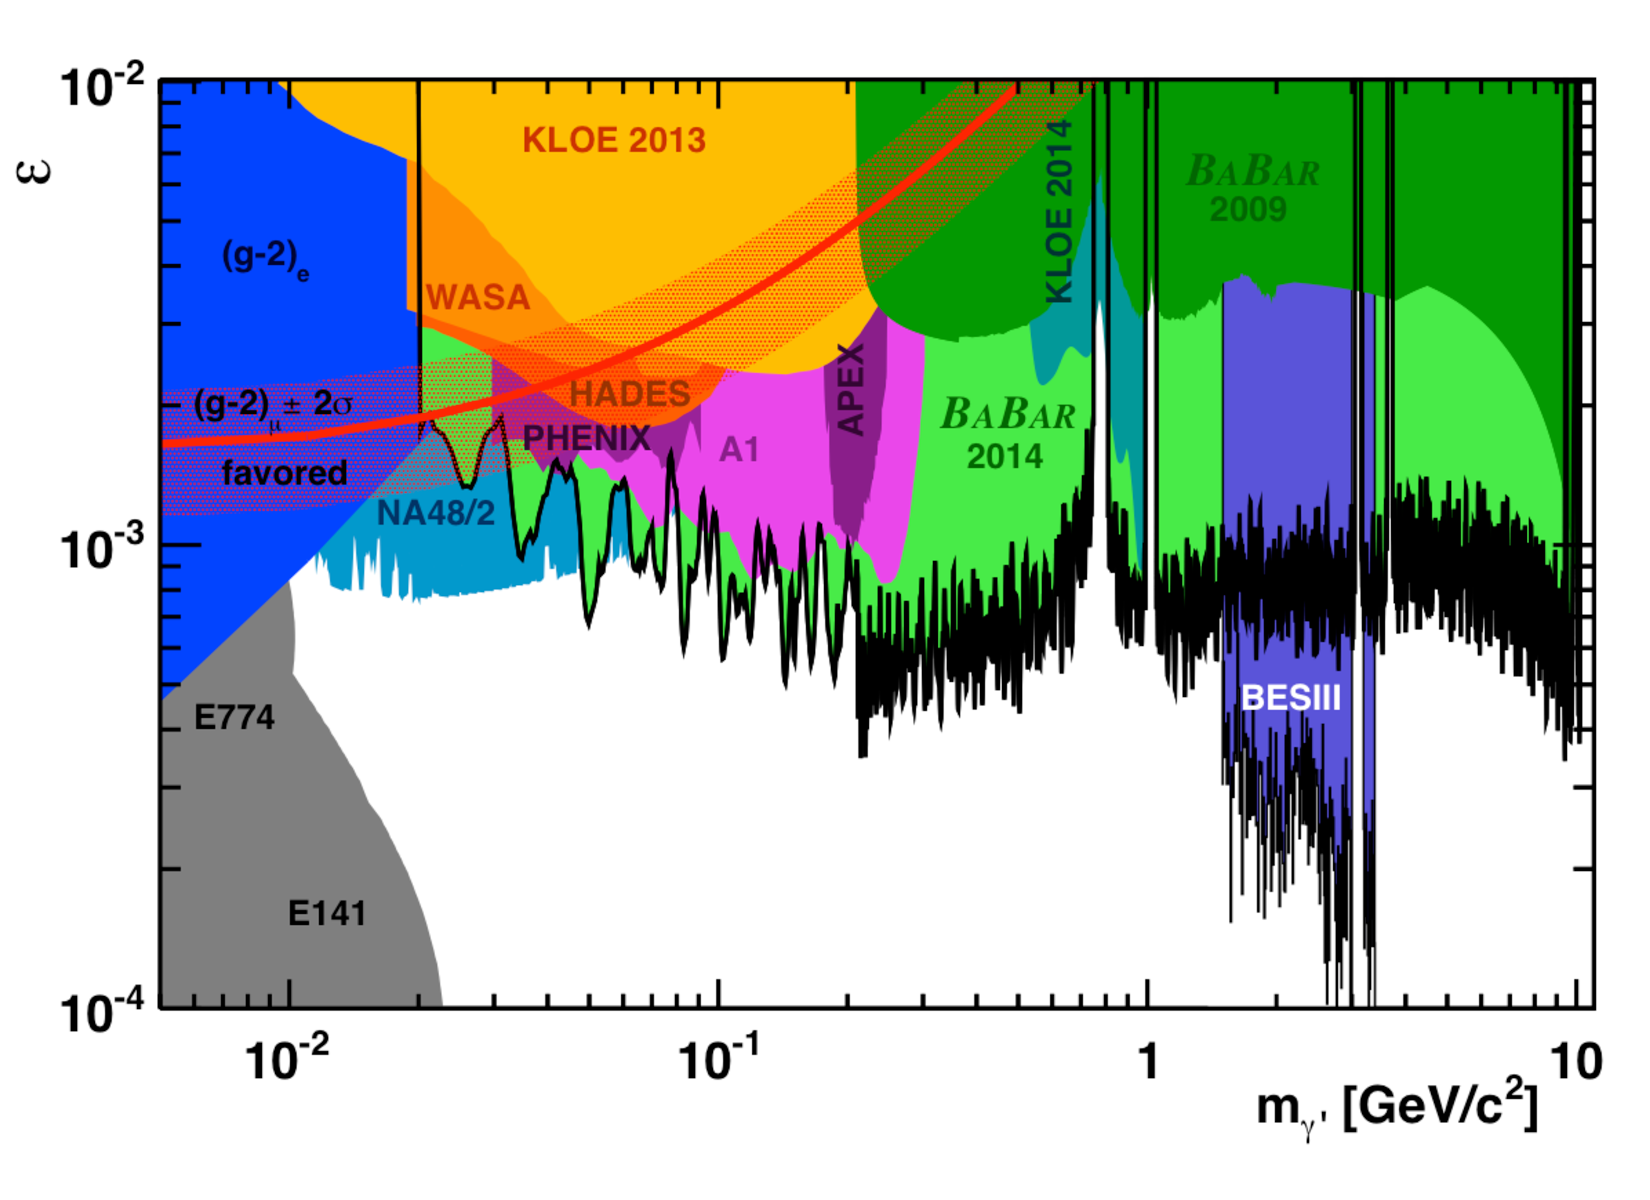
\includegraphics[width = 0.6\textwidth]{Figures/limits/darkphoton_limits}
    \caption{Current limits on the parameter space of the dark photon from \cite{Soffer:2015kpa}. The red band displays the region where the minimal dark photon model could explain $(g-2)_\mu$, and the dark blue region indicates the region ruled out by measurements of $(g-2)_e$. Recently NA48/2 has ruled out the possibility of the minimal model solving the anomalous magnetic moment of the muon.}
    \label{fig:darkphoton_limits}
\end{figure}

\subsection{Dark Scalar}
The Lagrangian we use for the addition of a scalar will replicate some features of the Higgs' Lagrangian after electroweak symmetry breaking, which couples to leptons.
We add a real scalar with Yukawa couplings to the three generations of mass, and a standard kinetic term, where the coupling strength is proportional to the mass of the lepton.
This obviously requires picking a mass scale for the coupling, one of two free parameters of the theory.
The other free parameter is, as usual, the mass of the new particle.
Choosing the coupling to scale proportionally to the mass may give a natural way to couple the new scalar more strongly to the $\mu$ than the $e$.
The full Lagrangian is given below,
\begin{equation}
\label{eqn:scalar_lagrangian}
\Lagr = \frac{1}{2}\partial_\mu \phi \partial^\mu \phi - \frac{1}{2} m_\phi^2 \phi^2 + \sum_{\ell=e,\mu,\tau} g_{\phi \ell}~\bar{\ell}^\lambda~\phi~\ell^\lambda + g_{\phi p}~\bar{p}~\phi~p + \Lagr_{\textrm{SM}}
% g_{\phi e}\bar{e}^\lambda e^\lambda \phi
\end{equation}
where $\ell$ takes on the lepton fields, the couplings in $g_{\phi \ell}$ are the couplings between the scalar and the corresponding lepton, $p$ is the proton field, $g_{\phi p}$ is the coupling between the scalar and the proton, $\Lagr_\textrm{SM}$ is the Standard Model Lagrangian, $\lambda$ indicates spinor indices, and $g_{\phi \ell} \propto m_\ell$.
We usually fix the coupling to the $\mu$ in this thesis, however we will also fix the coupling to the $\tau$ in one portion so it is convenient to write the couplings as:
\begin{equation*}
\label{eqn:coupling_mass}
g_{\phi \ell} = \left(g_{\phi e}, g_{\phi \mu}, g_{\phi \tau}\right) = g_{\phi \mu} \left( \frac{m_e}{m_\mu}, 1, \frac{m_\tau}{m_\mu} \right) = g_{\phi \tau} \left( \frac{m_e}{m_\tau}, \frac{m_\mu}{m_\tau}, 1 \right)
\end{equation*}

It is important to point out that this Lagrangian does not possess $SU(2) \times U(1)$ gauge invariance, as Yukawa interactions with leptons explicitly break this gauge symmetry. 
This hints that this theory is not UV complete, and at best represents a low-energy limit of a more consistent theory.
However, a UV complete version of this model, respecting $SU(2) \times U(1)$ gauge invariance, has been worked out which involves a SM neutral light scalar and a leptonic-specific two Higgs-doublet model \cite{Batell:2015unpub}.

With this model, the partial decay widths of the $\phi$ to pairs of leptons goes as

\begin{equation}
    \Gamma_{\phi \rightarrow \ell^+ \ell^-} = \frac{1}{8\pi^2} g_{\phi\ell}^2 m_\phi \left(1-\frac{4m_\ell^2}{m_\phi^2}\right)^{\frac{3}{2}}\textrm{.}
\end{equation}

If we examine the decay length to electrons, for masses of the mediator much larger than the electron, we find

\begin{equation}
    c \tau_{\phi \rightarrow e^+ e^-} \approx 0.16\textrm{mm} \left(\frac{10^{-4}}{g_{\phi e}}\right)^2 \frac{10\textrm{MeV}}{m_\phi}\textrm{.}
\end{equation}

\noindent The decay length is plotted in Fig.\ \ref{fig:ctau_phiee}.

\begin{figure}[h]
    \centering
    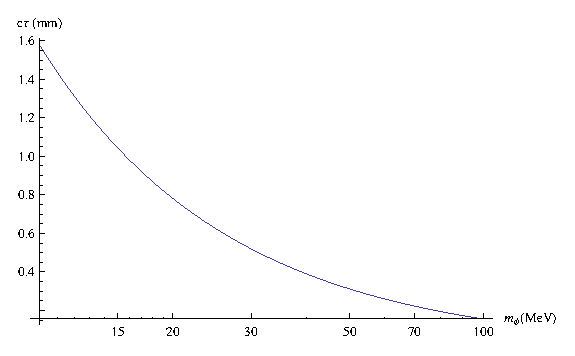
\includegraphics[width = 0.6\textwidth]{Figures/misc/ctau_phiee}
    \caption{The typical decay length of the scalar $\phi$, when electrons are the only lepton accessible. The strength of the coupling between $\phi$ and the electron is taken to be $g_{\phi e} = 10^{-4}$.}
    \label{fig:ctau_phiee}
\end{figure}

The largest implication of this decay width for us, is the relative partial widths between muons and electrons as the decay products.
Once the muon channel opens up, {\em i.e.}\ when $m_\phi > 2 m_\mu \gg 2 m_e$, and taking the total width to only have contributions from the $e^+ e^-$ and $\mu^+ \mu^-$ channels, we have that

\begin{align}
    \textrm{BR}(\phi \rightarrow \mu^+ \mu^-) &= \frac{1}{1+\frac{\Gamma\left(\phi \rightarrow e^+ e^-\right)}{\Gamma\left(\phi \rightarrow \mu^+ \mu^-\right)}} \\
    \frac{\Gamma_{\phi \rightarrow e^+ e^-}}{\Gamma_{\phi \rightarrow \mu^+ \mu^-}} &\approx \frac{m_e^2}{m_\mu^2}\left(1-\frac{4m_\mu^2}{m_\phi^2}\right)^{-\frac{3}{2}}\textrm{.}
\end{align}

\noindent Due to the suppression from the leading $m_e^2/m_\mu^2$ term, once the decay to muons is kinematically accessible due to the large mass of the $\phi$, one can effectively neglect the branching ratio to the electrons and take $\textrm{BR}(\phi \rightarrow \mu^+ \mu^-) \approx 1$.
A plot of the branching ratio to a dimuon pair is shown in Fig.\ \ref{fig:br_phimumu}.

\begin{figure}[h]
    \centering
    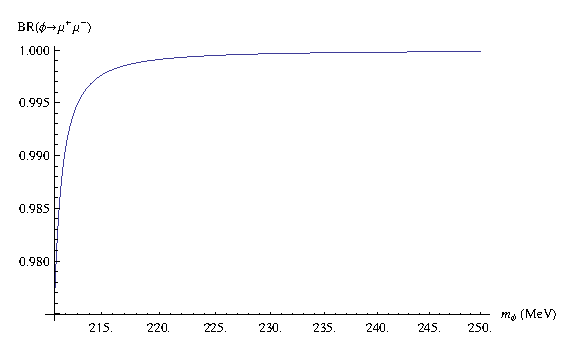
\includegraphics[width = 0.6\textwidth]{Figures/misc/br_phimumu}
    \caption{Typical branching ratios of the scalar $\phi$ to a dimuon pair. Here we have taken the coupling strength between the muon and the scalar to be $g_{\phi \mu} = 10^{-4}$. Going slightly above the threshold mass to produce pairs of muons gives a branching ratio of $1$ almost immediately.}
    \label{fig:br_phimumu}
\end{figure}

\noindent This has the consequence of allowing us to estimate sensitivity limits in an easier fashion, as we need only take into account the electron decay channel until the muon is accessible where it dominates, and similarly for the tau.
In all of our cases, we will be taking the $\phi$ to be produced on-shell before decaying to an $\ell^+ \ell^-$ pair promptly, as the width of the scalar as given above is very small, and the branching ratio to the most massive pair of leptons is very close to $1$.

Of most importance is the relative magnitude of couplings.
We would like a weak coupling to electrons such that we do not disturb the proton radius as extracted in the electron-proton scattering experiments, and measurement of the atomic energy levels of electronic Hydrogen.
Indeed the point here is to have a stronger coupling to the muon with the scalar, than that of the electron with the scalar.
Taking the couplings to be Higgs-like gives the size of any physical effect to be approximately some power of $(m_\mu/m_e) \approx 210$ times larger for the muon than to the electron.
Therefore, it is advantageous to produce such a scalar by radiating it off the heaviest lepton kinematically accessible in any given process.

It is also possible to allow for a pseudo-scalar coupling to be introduced, by introducing another set of couplings to the pseudo-scalar field and sandwiching an $i\gamma^5$ between spinors.
While it is outside the scope of this thesis to examine this, we will note here that the scalar and pseudo-scalar have corrections to the $(g-2)_\mu$ with opposing signs.
This is given in more detail in \cite{Carlson:2015jba}.

Since the phenomena we are trying to describe are the anomalous magnetic moment of the muon and the muonic atom's Lamb shift, we will discuss how the scalar model modifies these in detail.
The corrections to $(g-2)_\mu$ are given at the one loop level by \cite{Leveille:1977rc, McKeen:2009ny, TuckerSmith:2010ra}.
A convenient form for the contribution from the addition of a scalar is given below.

\begin{align}
    \Delta a_\mu &= \frac{\alpha}{2\pi} \left(\frac{g_{\phi\mu}}{e}\right)^2 \xi\left(\frac{m_\phi}{m_\mu}\right) \\
    \xi(x) &= \int_0^1 \frac{(1-z)^2(1+z)}{(1-z)^2 + x^2z} \,dz
\end{align}

\noindent This form of $\Delta a_\mu$ will be useful when plotting our proposed sensitivity limits.
For the case $m_\phi \ll m_\mu$, the integral $\xi \rightarrow 3/2$, giving an $m_\phi$ independent constraint on the coupling constant in this region.
When we are in the region $m_\phi \gg m_\mu$, the contribution at one loop scales as $\Delta a_\mu \propto (m_\mu/m_\phi)^2$, or similarly, the constraining coupling must scale as $g_{\phi\mu} \propto m_\phi / m)\mu$.
Overall we have the following asymptotic behaviour

\begin{equation}
    \Delta a_\mu = \frac{\alpha}{2\pi} \left(\frac{g_{\phi \mu}}{e}\right)^2
    \begin{cases}
        \frac{3}{2}, & m_\phi \ll m_\mu \\
        \frac{m_\mu^2}{m_\phi^2} \left(2\ln\left(\frac{m_\phi}{m_\mu}\right) - \frac{7}{6}\right), & m_\phi \gg m_\mu
    \end{cases}\textrm{,}
\end{equation}

\noindent and at a specific mass

\begin{equation}
    \Delta a_\mu\left(m_\phi = 50\textrm{MeV}\right) = \frac{\alpha}{2\pi} \left(\frac{g_{\phi\mu}}{10^{-4}}\right)^2 8.6\times 10^{-8}\textrm{.}
\end{equation}

The muonic atom's Lamb shift correction from the addition of a scalar can be found through first-order perturbation theory, and is given by \cite{TuckerSmith:2010ra, Carlson:2015jba}

\begin{align}
    \delta E_\phi &= \int r^2 V_\phi(r)\left(\left|R_{20}(r)\right|^2 - \left|R_{21}(r)\right|^2\right)\,dr \\
                  &= \frac{\alpha}{2 a^3} \left(\frac{g_{\phi\mu} g_{\phi p}}{e^2}\right) \frac{f(a m_\phi)}{m_\phi^2}
\end{align}

\noindent where $f(x) = x^4/(1+x)^4$, $a = 1/(\alpha m_{\mu p})$ is the Bohr radius of the $\mu\textrm{H}$ system, and $m_{\mu p}$ is the reduced mass of the system.
While it has proved to be a good motivation, and one can extract expected sensitivities with a constraint from the measurement of $r_p$, there is a degeneracy in this expression that proves difficult to work around.
Since the coupling to the proton must enter, we only see the product $g_{\phi\mu} g_{\phi p}$ enter in the above expression, which makes it difficult to place sensitivity limits on $g_{\phi\mu}$ without making assumptions on the coupling to the proton.
For this reason, $(g-2)_\mu$ proves to provide better context for the sensitivity limits we will explore.
